\documentclass[12pt]{book}
\usepackage{graphicx}
\usepackage[a4paper,inner=36mm,outer=18mm,top=30mm,]{geometry}
%\usepackage[doublespacing]{setspace} 
\usepackage{mathptmx}
\usepackage{siunitx}
\usepackage{titling}
\usepackage{amsmath}
\usepackage{hyperref}
\usepackage{gensymb}

\begin{document}

\title{Thesis}
\author{Emilio Dorigatti}

\maketitle

\section*{Summary}
todo

\tableofcontents

\chapter{Introduction}

\section{Problem}

Climatology, or climate science, studies the long-term average weather conditions. In the last few decades, climate scientists found solid evidence of ongoing changes in Earth's climate, most notably, a general increase in average temperature; in the long run, this and other changes can potentially have a devastating impact on life on our planet. Regardless of the causal effect of human activities on it, having a solid understanding of the climate allows us to find the best way to mitigate its change, and possibly prevent it completely.

Climate science is an extremely difficult field, for a number of reasons. First, climate is evident, by definition, only over long periods of time and large distances, making the usual scientific approach of testing hypotheses by conducting experiments inapplicable; instead, climate scientists have to rely on historical data. Second, the atmosphere is a complex and chaotic system, which must be described through systems of nonlinear differential equation. They can be used to create numerical simulations, and the resulting predictions compared to historical data to assess the accuracy of the theory. Furthermore, the chaotic character of the atmosphere makes it impossible to study parts of it in isolation from others, as small scale phenomena affect large scale ones, and vice versa. In spite of this, it is useful to split the atmosphere in vertical layers and horizontal zones, in order to differentiate among conditions and phenomena typically occurring in one area or the other.

Usually, the troposphere is referred to as the lowest layer of the atmosphere, but it can actually be subdivided in more sub-layers, the lowest of which is the \emph{atmospheric boundary layer}: it is the region of the atmosphere that is affected by the conditions of the surface. Most human activities happen in this layer, and it is responsible for a large part of the diffusion and transport of aerosol such as, among others, pollutants. Yet, the physics governing the atmospheric boundary layer is not fully understood, and the theory is lacking. One important issues in the study of the atmospheric boundary layer is the derivation of flux-profile relationships for wind and temperature: they essentially relate the transport of momentum and heat by the wind (flux) with the  change of wind speed/temperature with altitude (profile). The state of the art relationships are defined by the Monin-Obukhov Similarity theory in terms of the height above surface scaled by turbulence due to horizontal wind and vertical air movement due to variations in heat. Difficulties in measurements of relevant quantities make this theory accurate only up to 10-20\%, and applicable in a restricted set of conditions. 

In stark contrast to the traditional, top-down approach of science, recent developments in information technology made bottom-up approaches possible. In this new way of thinking, existing data is used to automatically infer the "best" explanation for the measurements at hand, the underlying laws that originated that data. The field that makes this possible is called Machine Learning: it takes advantage of several methods coming from statistics, information theory, optimization theory, etc., to make computers learn from examples. Together with Natural Language Processing and Automated Planning, it is one of the three main branches of Artificial Intelligence, the sub-field of Computer Science that studies ways of making machines behave intelligently.

todo more fluff about ml

\section{Research Question}
With the growing awareness of the shortcomings of the Monin-Obukhov similarity theory, and the recent availability of micro-meteorological data from specialized observation sites such as Cabauw, one naturally wonders whether the 

\section{Ethics and Sustainability}
todo

\section{Outline}
todo

\chapter{Background}
This chapter introduces the basic concepts the reader should be qualitatively familiar with, in order to understand the content of this thesis. It is assumed readers are already knowledgeable of simple mathematical concepts, such as calculus, linear algebra, statistics, and probability theory. Readers acquainted with the material should feel free to skip this chapter.

\section{Fluid Dynamics and the Boundary Layer}
Fluid dynamics is the discipline that studies the flow of fluids; it has several branches that study different fluids, such as aerodynamics (the study of air motion) and hydrodynamics (the study of water motion). These disciplines are routinely applied when designing cars, airplanes, ships, pipelines, etc.

\subsection{Laminar and Turbulent flow}
There are two distinct ways in which particles in a fluid can move: laminar flow and turbulent flow. In the former, all the particles move orderly, perhaps with a different speed, but all in the same direction, whereas in the latter the movement of particles is highly chaotic and unpredictable, and tends to dive rise to eddies of varying sizes. People are most familiar with the distinction between the two through the smoke rising from a cigarette, which starts smooth and becomes turbulent shortly thereafter, as in figure \ref{fig:smoke}. The kind of flow in under specific conditions can be predicted using the Reynolds number $Re$, which is the ratio between inertia forces, favoring turbulent flow, and viscosity forces, stabilizing the fluid towards laminar motion:

$$
Re=\frac{\rho u L}{\mu}=\frac{uL}{\nu}
$$

With $\rho$ the density of the fluid, $u$ its velocity, $L$ a characteristic linear dimension of the system under consideration, $\mu$ and $\nu$ the kinematic and dynamic viscosity of the fluid. The viscosity describes, intuitively, how much the molecules of the fluid tend to stick together and resist motion by generating drag. For example, water has low viscosity, and honey has high viscosity.

Since turbulence is random, it is usually studied in terms of the statistical properties of physical quantities through the Reynolds decomposition; given a quantity $a(s,t)$ which varies in space and time, we can compute its average

$$
\overline{a}(s)=\frac{1}{T}\int_{T_0}^{T_0+T}a(s,t)dt
$$

and the deviation from the average

$$
a'(s,t)=a(s,t)-\overline{a}(s)
$$

By definition, $\overline{a'}=0$, which means that all the effects of turbulence are contained in $a'$. Common statistical properties such as variance and covariance are expressed respectively as $\overline{a'a'}$ and $\overline{a'b'}$.

\begin{figure}
\caption{Smoke from a cigarette, and the transition from laminar to turbulent flow.}
\label{fig:smoke}
\centering
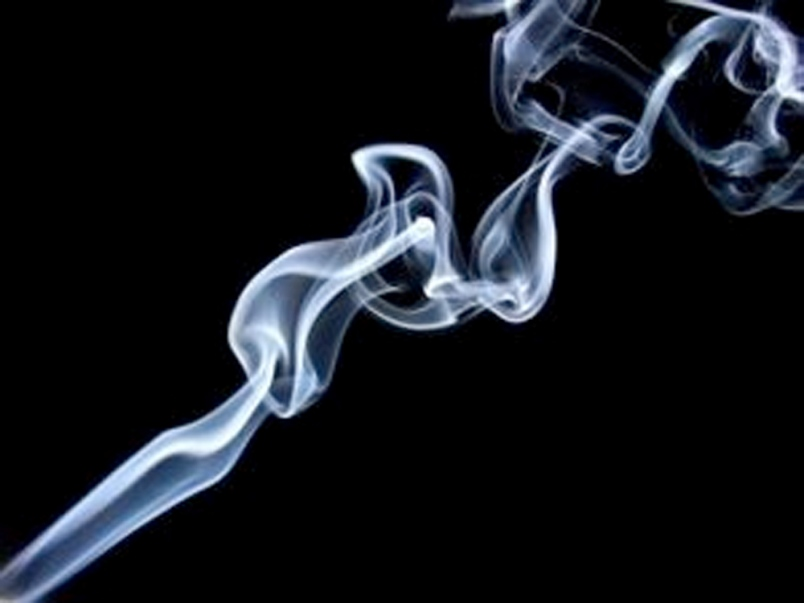
\includegraphics[width=0.5\textwidth]{images/smoke}
%https://www.google.se/search?client=ubuntu&q=cb+edits+smoke+png&tbm=isch&tbs=simg:CAQSlAEJkNL0D0I-7I0aiAELEKjU2AQaBAgVCAAMCxCwjKcIGl8KXQgDEiWoGUHnAegBsQw9sgxAlgawDIYnhSCHJ4okqzemIYgksCiVIKw3GjDJWGns8ZAx_17dvQFajhuRydFWdlJwDNo3VGI7iBUyNViewQZEJmiaYWGUhTUgxQOUgBAwLEI6u_1ggaCgoICAESBLt5JWoM&sa=X&ved=0ahUKEwiit7jKxKXZAhUBiCwKHTapCLQQ2A4IJygB&biw=1916&bih=948
\end{figure}


\section{The Boundary Layer}
In the context of fluid dynamics, the boundary layer studies the behavior of a fluid when it is flowing close to a solid surface. Imagine a laminar flow close to a solid surface; because of viscosity, the molecules flowing near the surface move slower, and, in the limit, the velocity of the molecules in direct contact with the surface is 0 (this is called the \emph{non-slip condition}). Thus, the velocity of the fluid increases smoothly, continuously and monotonously with the distance from the solid, until it reaches the \emph{free-flow} velocity, after which it stays constant. The region close to the surface, where the fluid moves slower, is called the \emph{boundary layer}, and is the region where the viscosity of the fluid influences its motion. Its height $\delta$ can be defined when the local velocity surpasses a certain threshold, such as 99\% of the free-flow velocity.

\begin{figure}
\caption{Turbulent boundary layer at the edge of a canal; the end of the BL is clearly visible, where the flow transitions from turbulent to laminar. Water flows from right to left.}
\label{fig:bl}
\centering
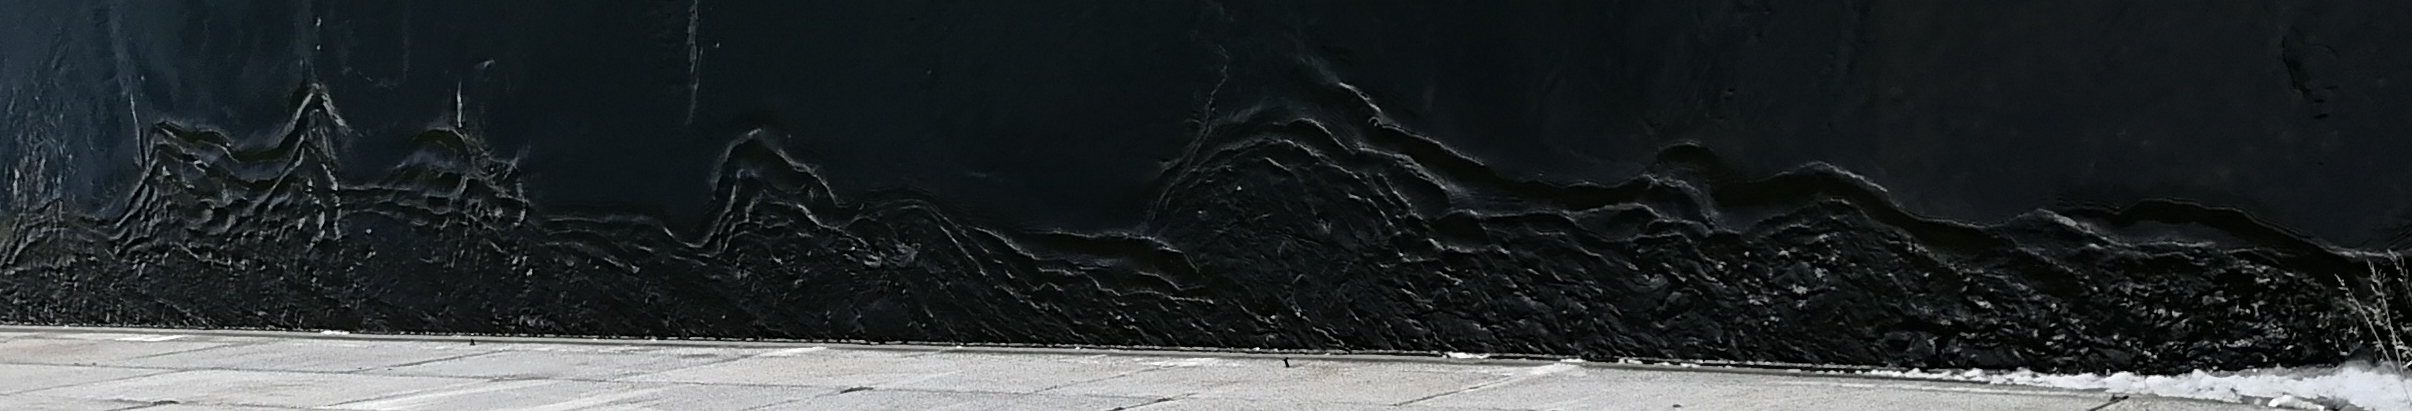
\includegraphics[width=\textwidth]{images/bl}
\end{figure}

The variation of velocity with distance from the surface, $\partial\overline{u}/\partial z$, is called \emph{shear}, and, together with viscosity, determines the materialization of turbulence in the flow. Every layer of fluid is squeezed between a faster moving layer above and a slower moving below; in high shear conditions, this causes high stress on the particles, and prevents them from moving orderly, thus leading to turbulent motion. Figure \ref{fig:bl} shows turbulence forming close to the wall in a canal, where the water flows from right to left. Viscosity and the no-slip condition prevent this phenomenon to arise in a region very close to the solid surface, called the \emph{laminar (or viscuous) sub-layer}, where we still find laminar motion.

The strength of the turbulence is proportional to $u_{rms}=(\overline{u'^2})^{1/2}$, which is, in turn, proportional to the shear. Again, because of the no-slip condition, $u_{rms}$ is zero at $z=0$, increases in the laminar sub-layer, and decreases to 0 at the end of the boundary layer, assuming laminar flow outside of it. Higher free-stream velocity generates higher shear, more turbulence, and a thinner laminar sub-layer. The strength of turbulence can be written in units of velocity, resulting in the \emph{friction velocity}, computed as $u_*=(\tau/\rho)^{1/2}=(\nu\cdot\partial\overline{u}/\partial z)^{1/2}$, where $\tau$ is the shear stress, $\rho$ is the density of the fluid, $\nu=\mu/\rho$ is the kinematic viscosity, and $\mu$ the dynamic viscosity. Therefore, the friction velocity increases with shear and viscosity, and decreases with density; it is proportional to the free-stream velocity and the turbulence strength, and inversely proportional to the height of the laminar sub-layer.

The mean velocity $\overline{u}$ increases linearly within the laminar sub-layer, then logarithmically until the end of the boundary layer, thus the shear decreases further away from the surface. In the logarithmic sub-layer, the velocity is computed as $\overline{u}(z)=u_*(\log z - \log z_0)/\kappa$, where $z_0$ is the characteristic roughness of the surface, and $\kappa$ is the von Karman's constant, whose value is around 0.4 [citation needed]. The characteristic roughness depends on the texture of the surface, and its relationship with the height $\delta_s$ of the laminar sub-layer; if the roughness scale is smaller than $\delta_s$, the logarithmic velocity profile is not affected by the texture, because the laminar sub-layer completely covers the variations on the surface, and we have the so-called smooth turbulent flow. If, on the contrary, the bumps in the surface are larger than $\delta_s$, the laminar sub-layer follow the profile of the surface, and the logarithmic velocity profile is altered depending on the texture, a regime called rough turbulent flow.

\section{The Atmospheric Boundary Layer}
The atmosphere is composed by air, which is behaves like fluid. Therefore, close to the Earth's surface, in the region called \emph{atmospheric boundary layer}, we find the same effects described in the previous section. Additionally, there are other phenomena that complicate things further, such as the temperature of the surface, which changes widely from day to night and from Summer to Winter, the rotation of the Earth, the varying roughness of the surface, due to cities and mountains, etc. The effect of the surface on the first few hundred meters of the atmosphere is the main focus of \emph{boundary layer meteorology}. 

The height of the atmospheric boundary layer (hereafter abbreviated as ABL) typically varies between 100 and 1000 meters, highly depending on the conditions, and it is always turbulent. There are three main instabilities driving turbulence in the ABL:

\begin{itemize}
\item Shear instability: caused by shear, the mechanism described in the previous section. This happens at high Reynolds number, and, by using typical values for the ABL, we find $Re$ well above $10^6$.
\item Kelvin-Helmholtz instability: occurs when there is a difference of density and velocity in different layers of flow. This is the mechanism that generates, for example, waves in ponds, lakes, and oceans.
\item Rayleigh-Bernard instability: is caused by the decrease of potential density\footnote{the potential density is the density that a parcel of air would attain if brought at a standard reference pressure adiabatically, i.e. disallowing exchanges of heat with its surroundings. Potential density is useful to compare densities irrespectively of pressure, i.e. altitude} with height, or, in other words, when warm fluid is below cold fluid; the warm fluid will rise, and the cold fluid will drop, a phenomenon called \emph{convection}. During hot Summer days, the surface is much warmer than the air, thus the air close to the surface will heat and tend to rise.
\end{itemize}

Turbulence has the very important role of transport and mix of air properties, such as heat, moisture, particles, aerosols, etc. This is especially true in \emph{unstable} conditions, when the air moving upwards (e.g. because it is warmer) is less dense than the air moving downwards; when the contrary happens, the ABL is called \emph{stable}.

The ABL can be divided in two main sub-layers: the inner surface layer and the outer Ekmann layer. This distinction is mainly done based on the scale of the dominating turbulent eddies: they are much smaller than the height of the ABL in the surface layer, and of comparable size in the outer layer.

It is very important to have a macroscopic understanding of the turbulent processes in the ABL, because they happen at length and time scales too small to be simulated in global climate models. The process of expressing the result of turbulence as a function of large scale parameters is called parametrization; having realistic models is essential in order to conduct precise simulations of the global climate in the scale of tens or hundreds of years, because errors tend to accumulate and amplificate as the simulation goes on. Other fields that benefit from the study of the ABL are urban meteorology (interested in the dispersion of pollutants), agricultural meteorology (interested in the formation of frost and dew, the temperature of the soil, etc.), aviation (predict fog and strong winds), and so on.

\subsection{Surface Fluxes}
A flux measures the amount of a physical quantity that flows through a surface. In the context of boundary layer meteorology, we are interested in the flows through the surface of earth, because, through them, the surface and the atmosphere exchange energy; these fluxes are thus measured in \si{\watt\per\square\meter}. The main source of energy for the surface is long-wave radiation coming from the sun, and short-wave radiation coming from the atmosphere and the clouds. A small amount of long-wave radiation is emitted from the surface, therefore let the net radiative flux be $R$, positive when the surface gains energy.

The main fluxes by which the surface loses energy to the atmosphere are called the turbulent flux of \emph{sensible heat} $H$, also called kinematic heat flux, and the turbulent flux of \emph{latent heat} $\lambda E$, also called kinematic flux of water vapor/moisture. The difference between the two is that the former causes an actual change of temperature, whereas the latter does not affect temperature\footnote{imagine a pot of boiling water; selecting a higher temperature on the stove will not increase the temperature of water above \SI{100}{\celsius}, but will make it boil faster. The additional heat introduced in the system is dissipated through increased evaporation}. The main causes of sensible heat fluxes are conduction and convection, whereas the main cause of latent heat fluxes is water movement: condensation, evaporation, melting, etc. 

The final flux of interest is the soil heat flux $G$, which is simply the heat "absorbed" by the surface and not given to the atmosphere. These four fluxes are linked by the surface energy balance equation:

$$
R=H+\lambda E+G
$$

which states that the total incoming energy $R$ must be equal to the energy given back to the atmosphere $H+\lambda E$ (not counting long-wave radiation, which is accounted to in $R$) plus the energy absorbed by the surface $G$.

The turbulent fluxes $H$ and $\lambda E$ are constant in the surface layer [todo add citation]. Experimentally, the energy balance is not always achieved [todo cite from cabauw] due to difficulty in measuring fluxes due to eddy correlation being inaccurate (verify this)

\subsection{The Turbulence Kinetic Energy Budged}
Kinetic energy is energy stored in form of movement: faster or heavier objects have more kinetic energy than slower or lighter ones. The Reynolds decomposition allows us to decompose the kinetic energy of turbulent flows in two terms: one caused by the mean flow, and one caused by turbulence. This decomposition can be justified by examining the temporal spectrum of kinetic energy, shown in figure \ref{fig:tkespectrum}. Four peaks are visible, corresponding to different sources of kinetic energy: turbulence, day-night cycle, westerlies\footnote{winds blowing from the east towards the west in the mid-latitudes}, and seasons. Importantly, there are few sources of kinetic energy in the 30 minutes to one hour time scale; this so-called spectral gap allows us to separate between turbulence and other sources of fluctuations in the atmosphere.

\begin{figure}
\caption{Change of atmospheric kinetic energy at different time-scales. The peaks in the scale of days and months and years are due to the day-night and Summer-Winter cycles, the peaks in the monthly scale are due to baroclinic instability in the mid-latitude westerlies, and the peaks at one minute are due to convection and atmospheric turbulence \cite{tkespectrumsrc,tkespectrumorig}}
\label{fig:tkespectrum}
\centering
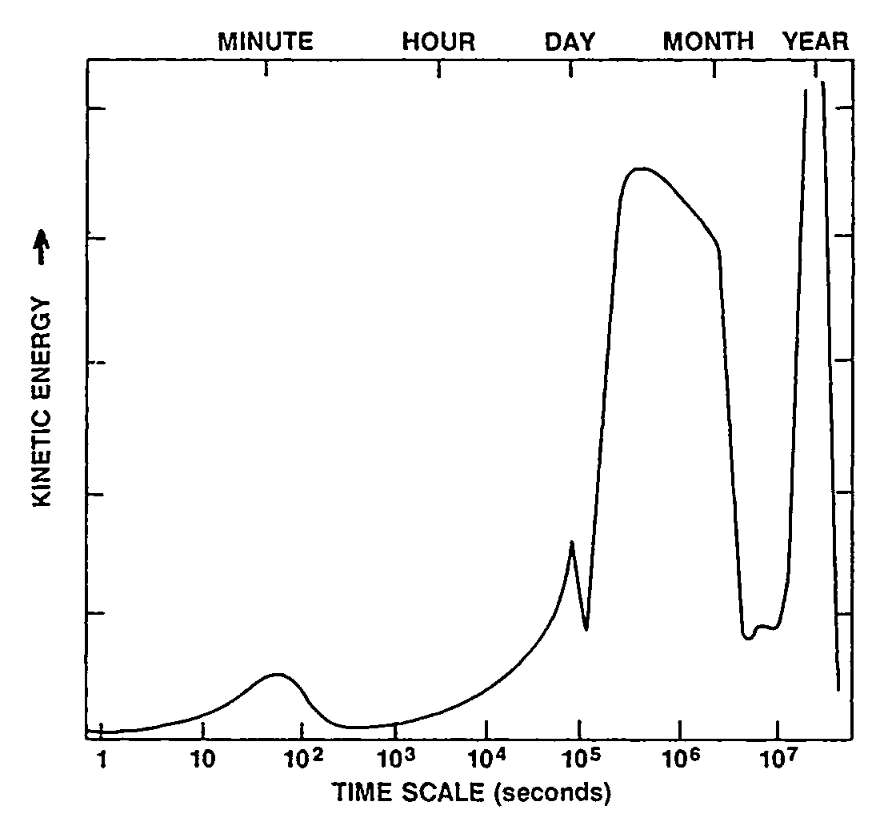
\includegraphics[width=0.5\textwidth]{images/kinetic_energy_spectrum}
\end{figure}

From now on, we will use a coordinate system with the $x$ axis aligned to the average horizontal wind direction, the $y$ axis perpendicular to it, and the $z$ axis pointing away from the surface. Then, we will use the letters $u$, $v$ and $w$ to denote the components of the wind along the axes $x$, $y$ and $z$ respectively; clearly, $\overline{v}=0$. Eddy fluxes can then be described in terms of covariances: let $\theta$ denote the potential temperature\footnote{the potential temperature is final temperature after bringing a parcel of air to a standard pressure adiabatically, i.e. not allowing exchange of temperature with the surroundings. It is a useful mean to compare temperatures irrespectively of pressure, i.e. altitude}, then $\overline{w'\theta'}$ is the turbulent heat flux, i.e. the sensible heat flux in the vertical due to wind. Usually the ABL  studied assuming homogeneous horizontal conditions, because they vary on a length scale larger than the height of the ABL. Because of this, the horizontal eddy correlations $\partial\overline{u'a'}/\partial x$ and $\partial\overline{v'a'}/\partial y$ are usually of negligible intensity, and are thus ignored. Note that this is not necessarily true when clouds are involved.

It is important to notice that turbulence is dissipative in nature. Consider a hot Summer day, where air is warmer close to the surface, and a circular eddy moving some air up and some down, so that the average motion is zero. The parcel of air moving up ($w'>0$) ends up being warmer than its surroundings ($\theta'>0$), while the one moving down ($w'<0$) will be colder ($\theta'<0$); the result is a new transport of heat through the eddy: $\overline{w'\theta'}>0$. On the contrary, imagine a cold night, where the air close to the surface is colder; the same eddy would transport a colder parcel of air upwards, and a warmer one downwards. In both cases, the end result would be a net transport of heat without transport of mass. Because of the ??? law, the eddy must lose energy, and thus dissipate over time.

Since turbulence changes over time, we are more interested in the change of kinetic energy, the turbulent kinetic energy budget. A full derivation is out of the scope of this work, but its final form \cite{basicatm} can be derived from prime physical principles, resulting in

$$
\frac{\partial\overline{{e'}^2}}{\partial t}
=\underbrace{\overline{u'w'}\frac{\partial\overline{u}}{\partial z}}_P
-\underbrace{\frac{g}{T}\overline{w'\theta'}}_B
+\underbrace{\frac{\partial}{\partial z}\frac{\overline{w'{e'}^2}}{2}}_{T_t}
+\underbrace{\frac{1}{\rho}\frac{\partial\overline{p'w'}}{\partial z}}_{T_p}
+\epsilon
$$

Where ${e'}^2={u'}^2+{v'}^2+{w'}^2$. The $P$ term is the production due to shear, $B$ is the production due to buoyancy (TODO why the negative sign?), $T_t$ is the turbulent transport of TKE (???), $T_p$ is the transport due to pressure, and $\epsilon$ is molecular dissipation due to viscosity.

TODO elaborate on 3.4, 3.5 (reason why P and B have opposite sign), 3.6, 

\subsection{Monin-Obukhov Similarity Theory}
One of the factors to distinguish laminar from turbulent flow is the length scale $L$ of the system. This length scale for the ABL was derived by A. M. Obukhov in 1946, and forms the basis of the similarity theory. According to this theory, the normalized wind and temperature profiles can be expressed as an unique function of $\xi=z/L$:

$$
L=-\frac{u_*^3}{\kappa\frac{g}{T_v}\frac{Q}{\rho c_\rho}}
=-\frac{u_*^3 T_v}{\kappa g \overline{w'\theta_v}}
$$

$$
\frac{\partial\overline{u}}{\partial z}\frac{kz}{u_*}=\phi_m(\xi)
$$

$$
\frac{\partial\overline{\theta}}{\partial z}\frac{kz}{T_*}=\phi_h(\xi)
$$

With

\begin{itemize}
\item $g=\SI{9.81}{\meter\per\square\second}$ the acceleration due to Earth's gravity
\item $\kappa=0.4$ the von Karman constant

\item $T_v$ virtual temperature\footnote{potential temperature of dry air if it had the same density as moist air. It allows to use formulas for dry air when the air is not dry.}, obtained as

$$
T_v=T\frac{1+r_v/\epsilon}{1+r_v}=T(1+0.61\cdot q)
$$

Where $r_v$ is the mixing ratio, $q=r_v/(1+r_v)$ the specific humidity, and $\epsilon$ is the ratio of the gas constants of dry air and water vapor, roughly 0.622.

\item $\rho$ the air density, computed from the pressure $P$ and the specific gas constant for dry air $R=\SI{287.058}{\joule\per\kilo\gram\kelvin}$ as

$$
\rho=\frac{P_0}{RT_v}
$$


\item $c_\rho$ specific heat of dry air, \SI{1005}{\joule\per\kilo\gram\per\kelvin} at \SI{300}{\kelvin}
\item $Q$ the buoyancy flux, approximated by $H+0.07\lambda E$ and measured in \si{\watt\per\square\meter}
\item $\overline{w'\theta_v}=Q/\rho c_\rho$ the flux of virtual potential temperature, measured in \si{\kelvin\meter\per\second}
\item $T_*=-\overline{w'\theta}/u_*$
\end{itemize}

The stability parameter $\xi$ is positive for stable conditions, where wind shear dominates the production of TKE, and negative for unstable conditions, where buoyancy is the main contributor to turbulence. It approaches 0 in the limit of neutral stratification (i.e. $\partial\overline{\theta}/\partial z=0$), because the temperature flux goes to 0 causing $L$ go to infinity.

The universal functions $\phi_m$ and $\phi_h$ must be determined experimentally. This is no easy task, and considerable effort has been devoted to it; one of the greatest difficulties lies in obtaining accurate and unbiased measurements, especially the fluxes. [hogstrom 1988] is a meta-study that aggregates and improves many previous results, and suggests the following expressions:

$$
\phi_m(\xi)=\begin{cases}
(1-19.3\xi)^{-1/4} & -2<\xi<0 \\
1+6\xi & 0<\xi<1\\
\end{cases}
$$

$$
\phi_h(\xi)=\begin{cases}
0.95(1-11.6\xi)^{-1/2} & -2<\xi<0 \\
0.95+8\xi & 0<\xi<1
\end{cases}
$$

The Monin-Obukhov similarity theory is only applicable in the surface layer, at heights much larger than the aerodynamic roughness length, and with $\vert\xi\vert<2$; even under ideal conditions, the predictions of this theory are accurate up to 10-20\% [foken 2006].

\section{ML stuff}
least squares, regularization, conjugate gradient, neural networks (?)

\subsection{Cross Validation}
true risk vs empirical risk, kfold, hkfold, nested cv

\chapter{Method}

\section{Data Collection}
The Cabauw Experimental Site for Atmospheric Research\footnote{\url{http://www.cesar-database.nl/}} (Cesar) is a consortium formed by eight Dutch institutes and universities, which collaborate to operate and maintain an observatory for micro-meteorological conditions near the village of Cabauw, the Netherlands. The data collected characterizes the state of the atmosphere and the soil, and their interaction via radiation and surface fluxes.

The observatory is surrounded by fields and no urban agglomerations is present within 15 kilometers; the land is flat with changes of altitude within a few meters over 20 kilometers. The main mast is 213 meters high and offers measurement levels every 20 meters; at each level there are three booms of length 10 meters that allow observations unobstructed by the main mast. There are three additional smaller masts of height 10 and 20 meters located close to the main mast, in order to obtain undisturbed measurements at the lower levels, and facilities to perform soil and surface observations.

The main focus of this project is on wind and temperature profiles, and the turbulent fluxes of sensible and latent heat. Additional variables, such as temperature and humidity, are needed to compute quantities of interest, most importantly the Obukhov length, and as possible predictors for the universal functions. There is one measurement for each variable every ten minutes, and missing measurements are gap-filled with a number of techniques. The data collected is always visually validated by an operator, which marks suspect or invalid sections of data

The Cesar observatory provides full information regarding data collection\footnote{\url{http://projects.knmi.nl/cabauw/insitu/observations/documentation}}, what follows is a brief summary of the most relevant sections.

\subsection{Wind Measurement}
Wind speed and direction are measured at heights of 200, 140, 80, 40, 20 and 10 meters, in either two or all three booms available. The wind vane that measures direction has a resolution of $1.5^\circ$, and the cup anemometer that measures wind speed has an accuracy of the largest between 1\% and \SI{0.1}{\meter\per\second}. The threshold sensitivity of both instruments is lower than \SI{0.5}{\meter\per\second}, and they report inaccurate measurements for up to \SI{3}{\meter\per\second} \cite{windinstr}.

For every ten minutes interval, the measurement comes from the instrument that is best exposed to the wind, and less affected by the obstruction caused by the mast. Corrections are then applied to the raw measurements to further attenuate the disturbance by the tower, following \cite{winddistortion}.

\subsection{Air Temperature Measurement}
Air temperature is measured at heights of 200, 140, 80, 40, 20, 10 and 1.5 meters

\subsection{Eddy Correlation}
The eddy correlation technique is used to compute the turbulent surface fluxes of sensible and latent heat, as well as momentum and $CO_2$, starting from fluctuations in wind, temperature, and humidity.

These measurements are obtained with, respectively, a sonic anemometer, a sonic thermometer, and an optical open-path sensor. Sonic anemometers measure the wind speed by leveraging the fact that the speed of sound in free air is affected by the speed of the air itself; since the speed of sound is known, the wind speed can be easily recovered from the time a sound impulse takes to travel a short distance. By measuring the wind velocity along three orthogonal paths, the full wind vector can be recovered. Sonic thermometers work similarly, by leveraging the fact that the speed of sound is affected by the temperature of the medium it travels in. These instruments can take up to 100 measurements per second. Optical open-path sensors quantify the amount of water vapor and carbon dioxide in the air by emitting a ray of infrared light and measuring its intensity 10 to 20 centimeters further away. $H_2O$ and $CO_2$ molecules in the air absorb electromagnetic radiation at known frequencies, thus the concentration of water vapor and carbon dioxide can be inferred by measuring the attenuation at these wavelengths.

The eddy correlation technique measures fluxes by computing their sample covariance with the vertical wind speed. Let $w_t$ be the vertical wind speed at time $t$, then the turbulent vertical flux for the quantity $a$ is computed as follows:

$$
F_a=\frac{1}{T_2-T_1}\sum_{t=T_1}^{T_2}(w_t-\overline{w})(a_t-\overline{a})
$$

Where $\overline{w}$ and $\overline{a}$ are the averages of $w_t$ and $a_t$ for $T_1\leq t\leq T_2$. The fluxes in the Cesar database are computed every ten minutes, with 10 measurements per second.

The eddy correlation technique is far from perfect, see \cite{microhandbook} for a detailed summary of issues.

\subsection{Gap Filling}
With gap-filling, missing measurements are replaced by synthetic values. The gap-filling method depends on the missing parameter and the duration of the period where data is not available. There are two classes of parameters: forcing parameters, which include wind, temperature, specific humidity, incoming radiation and rain, and validation parameters, which include the surface fluxes, outgoing radiation, and friction velocity.

For less than two hours of missing measurements, both forcing and evaluation parameters are gap-filled by interpolation of nearby values. For longer periods, forcing parameters are derived by transforming measures obtained from the nearby site of De Bilt, which are themselves gap-filled. Evaluation parameters are computed with a vegetation model that uses the forcing parameters as input.


\section{Monin-Obukhov Similarity Theory}
talk about recreating MOST with data from cabauw (and possibly arm)

\subsection{Profile Computation}
get gradient from measures

\subsection{Model Fitting}
get coefficients from our data

\chapter{Results}
todo

\chapter{Discussion}
todo

\section{Limitations and Future Work}
todo

\bibliographystyle{unsrt}
\bibliography{thesis}

\end{document}
